\documentclass[10pt]{article}\usepackage[]{graphicx}\usepackage[]{color}
%% maxwidth is the original width if it is less than linewidth
%% otherwise use linewidth (to make sure the graphics do not exceed the margin)
\makeatletter
\def\maxwidth{ %
  \ifdim\Gin@nat@width>\linewidth
    \linewidth
  \else
    \Gin@nat@width
  \fi
}
\makeatother

\definecolor{fgcolor}{rgb}{0.345, 0.345, 0.345}
\newcommand{\hlnum}[1]{\textcolor[rgb]{0.686,0.059,0.569}{#1}}%
\newcommand{\hlstr}[1]{\textcolor[rgb]{0.192,0.494,0.8}{#1}}%
\newcommand{\hlcom}[1]{\textcolor[rgb]{0.678,0.584,0.686}{\textit{#1}}}%
\newcommand{\hlopt}[1]{\textcolor[rgb]{0,0,0}{#1}}%
\newcommand{\hlstd}[1]{\textcolor[rgb]{0.345,0.345,0.345}{#1}}%
\newcommand{\hlkwa}[1]{\textcolor[rgb]{0.161,0.373,0.58}{\textbf{#1}}}%
\newcommand{\hlkwb}[1]{\textcolor[rgb]{0.69,0.353,0.396}{#1}}%
\newcommand{\hlkwc}[1]{\textcolor[rgb]{0.333,0.667,0.333}{#1}}%
\newcommand{\hlkwd}[1]{\textcolor[rgb]{0.737,0.353,0.396}{\textbf{#1}}}%
\let\hlipl\hlkwb

\usepackage{framed}
\makeatletter
\newenvironment{kframe}{%
 \def\at@end@of@kframe{}%
 \ifinner\ifhmode%
  \def\at@end@of@kframe{\end{minipage}}%
  \begin{minipage}{\columnwidth}%
 \fi\fi%
 \def\FrameCommand##1{\hskip\@totalleftmargin \hskip-\fboxsep
 \colorbox{shadecolor}{##1}\hskip-\fboxsep
     % There is no \\@totalrightmargin, so:
     \hskip-\linewidth \hskip-\@totalleftmargin \hskip\columnwidth}%
 \MakeFramed {\advance\hsize-\width
   \@totalleftmargin\z@ \linewidth\hsize
   \@setminipage}}%
 {\par\unskip\endMakeFramed%
 \at@end@of@kframe}
\makeatother

\definecolor{shadecolor}{rgb}{.97, .97, .97}
\definecolor{messagecolor}{rgb}{0, 0, 0}
\definecolor{warningcolor}{rgb}{1, 0, 1}
\definecolor{errorcolor}{rgb}{1, 0, 0}
\newenvironment{knitrout}{}{} % an empty environment to be redefined in TeX

\usepackage{alltt}

\usepackage{amsmath,amssymb,amsthm}
\usepackage{fancyhdr,url}
\usepackage{graphicx}

\oddsidemargin 0in  %0.5in
\topmargin     0in
\leftmargin    0in
\rightmargin   0in
\textheight    9in
\textwidth     6in %6in
%\headheight    0in
%\headsep       0in
%\footskip      0.5in


\pagestyle{fancy}

\lhead{\textsc{Prof. McNamara}}
\chead{\textsc{SDS/MTH 220: Lecture Notes}}
\rhead{\textsc{April 19, 2017}}
\lfoot{}
\cfoot{}
%\cfoot{\thepage}
\rfoot{}
\renewcommand{\headrulewidth}{0.2pt}
\renewcommand{\footrulewidth}{0.0pt}

\newcommand{\ans}{\vspace{1in}}
\IfFileExists{upquote.sty}{\usepackage{upquote}}{}
\begin{document}
%\maketitle

\paragraph{Agenda}
\begin{enumerate}
  \itemsep0em 
  \item Inference for multiple regression
  \item More regression diagnostics
  \item Bootstrap for regression
\end{enumerate}

% \paragraph{Case study: Predictors of depressive symptoms}
% 
% In the HELP (Health Evaluation and Linkage to Primary Care) study, investigators were interested in determining predictors of severe depressive symptoms (measured by the Center for Epidemiologic Studies - Depression scale, aka {\tt cesd}) amongst a cohort enrolled at a substance abuse treatment facility. These includes {\tt substance} of abuse (alcohol, cocaine, or heroin), {\tt mcs} (a measure of mental well-being), gender and housing status (housed or homeless). Consider the following multiple regression model.
% 
% <<message=FALSE, eval=TRUE, size='scriptsize', warning=FALSE>>=
% library(mosaic)
% fm <- lm(cesd ~ substance + mcs + sex + homeless, data = HELPrct)
% msummary(fm)
% confint(fm)
% @
% 
% 
% <<size='footnotesize',fig.height=4,fig.width=10, echo=FALSE>>=
% plot1 = histogram(~ residuals(fm), xlab="residuals", fit="normal")
% plot2 = xyplot(residuals(fm) ~ fitted(fm), xlab="fitted values", ylab="residuals",
%   type=c("p", "r", "smooth"))
% plot3 = xyplot(residuals(fm) ~ mcs, xlab="Mental Component Score", ylab="residuals", 
%   type=c("p", "r", "smooth"), data=HELPrct)
% print(plot1, position=c(0, 0, 1/3, 1), more=TRUE)
% print(plot2, position=c(1/3, 0, 2/3, 1), more=TRUE)
% print(plot3, position=c(2/3, 0, 1, 1))
% @
% 
% \begin{enumerate}
% \itemsep0.9in
% \item Write out the linear model
% \item Calculate the predicted CESD for a female homeless cocaine-involved subject with
% an MCS score of 20.
% %\item Identify the null and alternative hypotheses for the 8 tests displayed above
% 
% \item Interpret the 95\% confidence interval for the {\tt substancecocaine} coefficient
% 
% \item Make a conclusion and summarize the results of a test of the {\tt homeless} parameter
% \item Report and interpret the $R^2$ (coefficient of determination) for this model
% %\item Which of the residual diagnostic plots are redundant?  
% \item What do we conclude about the distribution of the residuals?
% \item What do we conclude about the relationship between the fitted values and the residuals?
% \item What do we conclude about the relationship between the MCS score and the residuals?
% \item What other things can we learn from the residual diagnostics?
% \item Which observations should we flag for further study?
% \end{enumerate}
% 
% 
% <<size='footnotesize', eval=FALSE>>=
% help_mod <- broom::augment(fm)
% help_mod %>%
%   slice(c(40, 351, 433, 450))
% @
% 
% \newpage

\paragraph{Case Study: Gestation redux}

The Child Health and Development Studies investigate a range of topics. One study, in particular, considered all pregnancies between 1960 and 1967 among women in the Kaiser Foundation Health Plan in the San Francisco East Bay area. The goal is to model the weight of the infants (\texttt{bwt}, in ounces) using variables including length of pregnancy in days (\texttt{gestation}), mother's age in years (\texttt{age}), mother's height in inches (\texttt{height}), whether the child was the first born (\texttt{parity}), mother's pregnancy weight in pounds (\texttt{weight}), and whether the mother was a smoker (\texttt{smoke}). 
The summary table below shows the results of a regression model for predicting the average birth weight of babies based on all of the variables included in the data set.

\begin{knitrout}\footnotesize
\definecolor{shadecolor}{rgb}{0.969, 0.969, 0.969}\color{fgcolor}\begin{kframe}
\begin{alltt}
\hlkwd{library}\hlstd{(mosaic)}
\hlstd{mod} \hlkwb{<-} \hlkwd{lm}\hlstd{(wt} \hlopt{~} \hlstd{gestation} \hlopt{+} \hlstd{age} \hlopt{+} \hlstd{ht} \hlopt{+} \hlstd{wt.1} \hlopt{+} \hlstd{parity} \hlopt{+} \hlstd{smoke,} \hlkwc{data} \hlstd{= Gestation)}
\hlkwd{msummary}\hlstd{(mod)}
\end{alltt}
\begin{verbatim}
##              Estimate Std. Error t value Pr(>|t|)    
## (Intercept) -88.70273   14.85467  -5.971 3.12e-09 ***
## gestation     0.46317    0.03013  15.371  < 2e-16 ***
## age           0.02450    0.09681   0.253   0.8002    
## ht            1.09399    0.21266   5.144 3.15e-07 ***
## wt.1          0.06067    0.02628   2.309   0.0211 *  
## parity        0.56354    0.30092   1.873   0.0614 .  
## smoke        -0.88334    0.52846  -1.672   0.0949 .  
## 
## Residual standard error: 16.35 on 1167 degrees of freedom
##   (62 observations deleted due to missingness)
## Multiple R-squared:  0.2087,	Adjusted R-squared:  0.2046 
## F-statistic: 51.29 on 6 and 1167 DF,  p-value: < 2.2e-16
\end{verbatim}
\begin{alltt}
\hlkwd{confint}\hlstd{(mod)}
\end{alltt}
\begin{verbatim}
##                     2.5 %      97.5 %
## (Intercept) -1.178476e+02 -59.5578925
## gestation    4.040487e-01   0.5222936
## age         -1.654278e-01   0.2144369
## ht           6.767417e-01   1.5112356
## wt.1         9.108466e-03   0.1122317
## parity      -2.687411e-02   1.1539491
## smoke       -1.920186e+00   0.1535040
\end{verbatim}
\end{kframe}
\end{knitrout}

\begin{enumerate}
  \itemsep0.7in
  \item Write the equation of the regression line that includes all of the variables.
  \item Interpret the slopes of \texttt{gestation} and \texttt{age} in this context.
  \item Identify the null and alternative hypotheses for the 6 tests displayed above. 
  \newpage
  \item Interpret the 95\% confidence interval for the {\tt smoke} coefficient
  \item The coefficient for \texttt{parity} is different than if you fit a linear model predict weight using only that variable. Why might there be a difference?
\begin{knitrout}\footnotesize
\definecolor{shadecolor}{rgb}{0.969, 0.969, 0.969}\color{fgcolor}\begin{kframe}
\begin{alltt}
\hlkwd{coef}\hlstd{(}\hlkwd{lm}\hlstd{(wt} \hlopt{~} \hlstd{parity,} \hlkwc{data} \hlstd{= Gestation))}
\end{alltt}
\begin{verbatim}
## (Intercept)      parity 
## 119.0369557   0.2794484
\end{verbatim}
\end{kframe}
\end{knitrout}
  
  \item Calculate the residual for the first observation in the data set.
\begin{knitrout}\footnotesize
\definecolor{shadecolor}{rgb}{0.969, 0.969, 0.969}\color{fgcolor}\begin{kframe}
\begin{alltt}
\hlkwd{head}\hlstd{(Gestation,} \hlnum{1}\hlstd{)}
\end{alltt}
\begin{verbatim}
##   id pluralty outcome date gestation sex  wt parity race age ed ht wt.1
## 1 15        5       1 1411       284   1 120      1    8  27  5 62  100
##   drace dage ded dht dwt marital inc smoke time number
## 1     8   31   5  65 110       1   1     0    0      0
\end{verbatim}
\begin{alltt}
\hlcom{# head(fitted(mod), 1)}
\hlcom{# head(residuals(mod), 1)}
\end{alltt}
\end{kframe}
\end{knitrout}
  
  \item The variance of the residuals is 249.28, and the variance of the birth weights of all babies in the data used to build the model is 335.94. Calculate the $R^2$ and the adjusted $R^2$. Note that there are 1236 observations in the data set, but there was missing data in 62 of those observations, so only 1174 observations were used to build the regression model.
  
\begin{knitrout}\footnotesize
\definecolor{shadecolor}{rgb}{0.969, 0.969, 0.969}\color{fgcolor}\begin{kframe}
\begin{alltt}
\hlkwd{var}\hlstd{(}\hlopt{~}\hlkwd{residuals}\hlstd{(mod))}
\end{alltt}
\begin{verbatim}
## [1] 265.8434
\end{verbatim}
\begin{alltt}
\hlkwd{var}\hlstd{(}\hlopt{~}\hlstd{wt,} \hlkwc{data} \hlstd{= mod}\hlopt{$}\hlstd{model)}
\end{alltt}
\begin{verbatim}
## [1] 335.9402
\end{verbatim}
\begin{alltt}
\hlcom{# rsquared(mod)}
\end{alltt}
\end{kframe}
\end{knitrout}
 \newpage
  \item This data set contains missing values. What happens to these rows? 
  \item Interpret the $R^2$ (coefficient of determination) for this model
  \vspace{0.7in}
\end{enumerate}





\paragraph{Regression Diagnostics}

\begin{itemize}
  \itemsep0em
  \item \textbf{L}inearity-- scatterplot (only in s.l.r.), residual vs. fitted plot
  \item \textbf{I}ndependence-- the thinking condition
  \item \textbf{N}ormality (of residuals)-- QQ plot or histogram of residuals
  \item \textbf{E}qual Variance (of residuals)-- residual vs. fitted plot
\end{itemize}  
\begin{itemize}
  \item Investigate outliers and influentional points
  \item Investigate possible multicollinearity
\end{itemize}

\paragraph{Residual analysis} 

You can roll your own:

\begin{knitrout}\footnotesize
\definecolor{shadecolor}{rgb}{0.969, 0.969, 0.969}\color{fgcolor}\begin{kframe}
\begin{alltt}
\hlstd{babies_mod} \hlkwb{=} \hlstd{broom}\hlopt{::}\hlkwd{augment}\hlstd{(mod)}
\hlkwd{qplot}\hlstd{(}\hlkwc{y} \hlstd{= .resid,} \hlkwc{x} \hlstd{= .fitted,} \hlkwc{data} \hlstd{= babies_mod)} \hlopt{+} \hlkwd{geom_smooth}\hlstd{()}
\hlkwd{qplot}\hlstd{(}\hlkwc{y} \hlstd{= .resid,} \hlkwc{x} \hlstd{= gestation,} \hlkwc{data} \hlstd{= babies_mod)} \hlopt{+} \hlkwd{geom_smooth}\hlstd{()}
\hlkwd{qplot}\hlstd{(}\hlkwc{y} \hlstd{= .resid,} \hlkwc{x} \hlstd{= age,} \hlkwc{data} \hlstd{= babies_mod)} \hlopt{+} \hlkwd{geom_smooth}\hlstd{()}
\hlkwd{qplot}\hlstd{(}\hlkwc{y} \hlstd{= .resid,} \hlkwc{x} \hlstd{= ht,} \hlkwc{data} \hlstd{= babies_mod)} \hlopt{+} \hlkwd{geom_smooth}\hlstd{()}
\hlkwd{qplot}\hlstd{(}\hlkwc{y} \hlstd{= .resid,} \hlkwc{x} \hlstd{= wt.1,} \hlkwc{data} \hlstd{= babies_mod)} \hlopt{+} \hlkwd{geom_smooth}\hlstd{()}
\hlkwd{qplot}\hlstd{(}\hlkwc{sample} \hlstd{= .resid,} \hlkwc{data} \hlstd{= babies_mod,} \hlkwc{geom} \hlstd{=} \hlstr{"qq"}\hlstd{)}
\hlkwd{qplot}\hlstd{(}\hlkwc{x} \hlstd{= .resid,} \hlkwc{data} \hlstd{= babies_mod,} \hlkwc{geom} \hlstd{=} \hlstr{"blank"}\hlstd{)} \hlopt{+}
  \hlkwd{geom_histogram}\hlstd{(}\hlkwd{aes}\hlstd{(}\hlkwc{y} \hlstd{= ..density..),} \hlkwc{binwidth} \hlstd{=} \hlnum{4}\hlstd{)} \hlopt{+}
  \hlkwd{stat_function}\hlstd{(}\hlkwc{fun} \hlstd{= dnorm,} \hlkwc{args} \hlstd{=} \hlkwd{c}\hlstd{(}\hlkwc{mean} \hlstd{=} \hlnum{0}\hlstd{,} \hlkwc{sd} \hlstd{=} \hlkwd{sd}\hlstd{(babies_mod}\hlopt{$}\hlstd{.resid)),} \hlkwc{col} \hlstd{=} \hlstr{"tomato"}\hlstd{)}
\end{alltt}
\end{kframe}
\end{knitrout}

Or use the built-in diagnostics:

\begin{knitrout}\footnotesize
\definecolor{shadecolor}{rgb}{0.969, 0.969, 0.969}\color{fgcolor}\begin{kframe}
\begin{alltt}
\hlkwd{plot}\hlstd{(mod,} \hlkwc{which}\hlstd{=}\hlkwd{c}\hlstd{(}\hlnum{1}\hlstd{,}\hlnum{2}\hlstd{))}
\end{alltt}
\end{kframe}
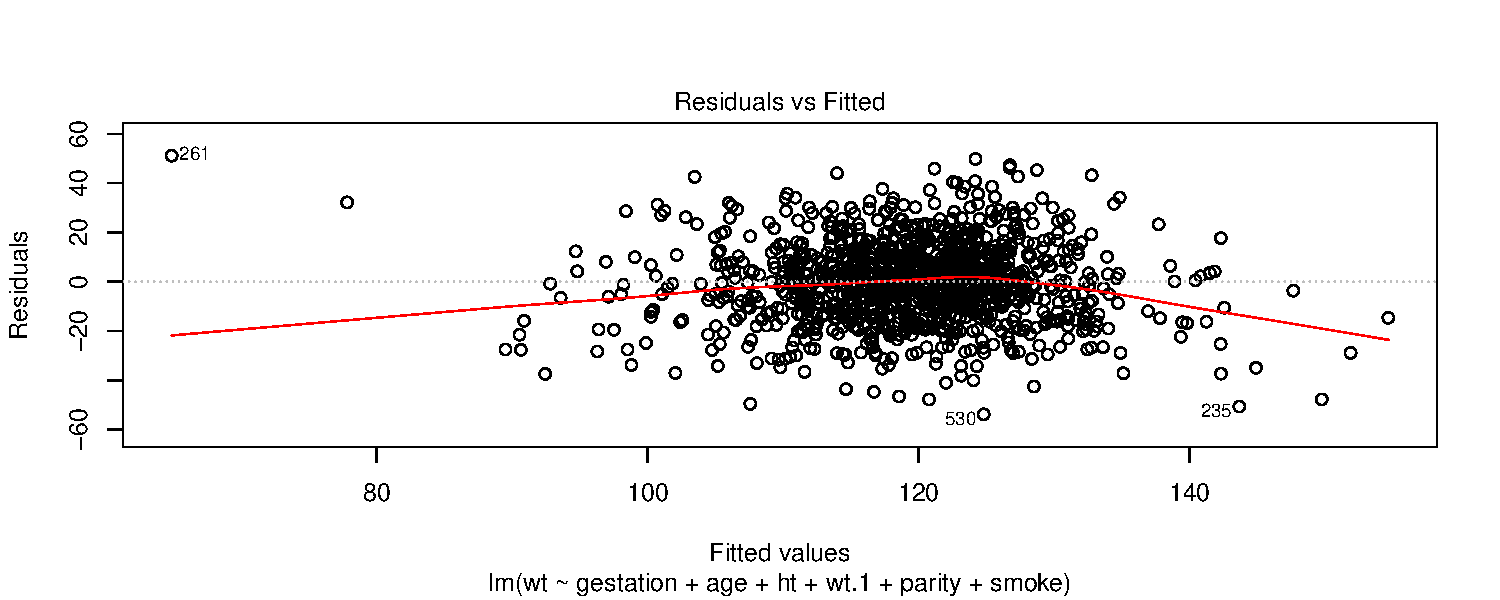
\includegraphics[width=\maxwidth]{figure/unnamed-chunk-6-1} 

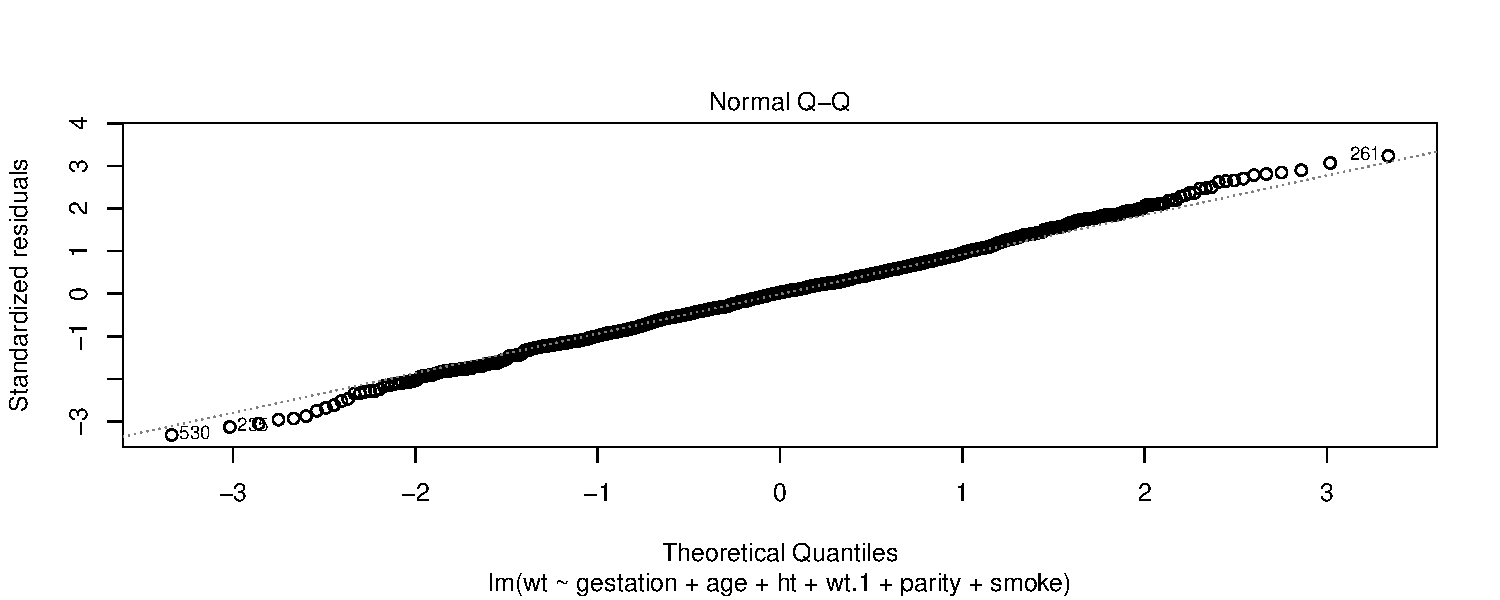
\includegraphics[width=\maxwidth]{figure/unnamed-chunk-6-2} 

\end{knitrout}

What do you think about the conditions for this model? Are they upheld?

\paragraph{Interesting observations} Are there interesting individual observations?

\begin{knitrout}\footnotesize
\definecolor{shadecolor}{rgb}{0.969, 0.969, 0.969}\color{fgcolor}\begin{kframe}
\begin{alltt}
\hlkwd{glimpse}\hlstd{(}\hlkwd{slice}\hlstd{(Gestation,} \hlkwd{c}\hlstd{(}\hlnum{261}\hlstd{,} \hlnum{235}\hlstd{)))}
\end{alltt}
\begin{verbatim}
## Observations: 2
## Variables: 23
## $ id        <int> 4604, 3863
## $ pluralty  <int> 5, 5
## $ outcome   <int> 1, 1
## $ date      <int> 1598, 1610
## $ gestation <int> 148, 318
## $ sex       <int> 1, 1
## $ wt        <int> 116, 93
## $ parity    <int> 7, 7
## $ race      <int> 7, 7
## $ age       <int> 28, 31
## $ ed        <int> 1, 0
## $ ht        <int> 66, 66
## $ wt.1      <int> 135, 135
## $ drace     <fctr> 7, 7
## $ dage      <int> 36, 30
## $ ded       <int> 1, 4
## $ dht       <int> 68, NA
## $ dwt       <int> 155, NA
## $ marital   <int> 0, 1
## $ inc       <int> 2, NA
## $ smoke     <int> 0, 0
## $ time      <int> 0, 0
## $ number    <int> 0, 0
\end{verbatim}
\end{kframe}
\end{knitrout}


\paragraph{Multicolinearity} Are there strong \emph{pairwise} correlations between any of the explanatory variables?

\begin{knitrout}\footnotesize
\definecolor{shadecolor}{rgb}{0.969, 0.969, 0.969}\color{fgcolor}\begin{kframe}
\begin{alltt}
\hlkwd{library}\hlstd{(GGally)}
\hlstd{nbabies} \hlkwb{<-} \hlstd{Gestation} \hlopt
  \hlkwd{select}\hlstd{(gestation, age, ht, wt.1)}
\hlkwd{ggpairs}\hlstd{(nbabies)}
\end{alltt}
\end{kframe}
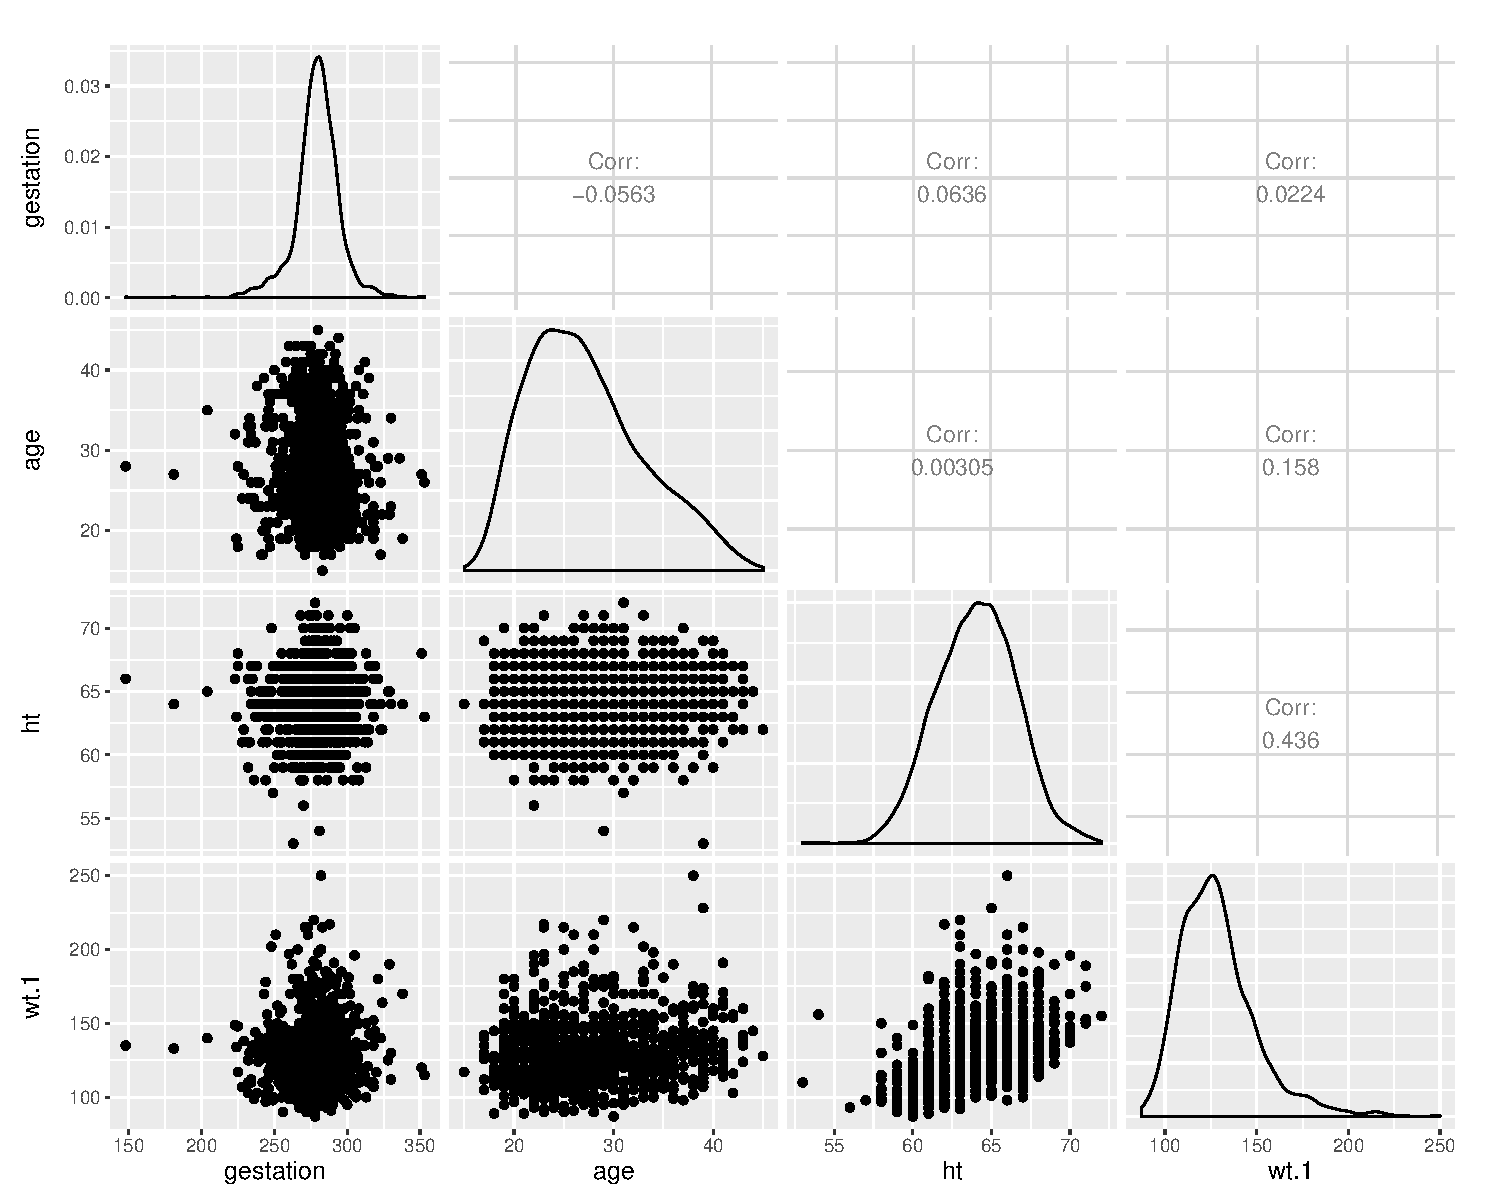
\includegraphics[width=\maxwidth]{figure/unnamed-chunk-8-1} 

\end{knitrout}


\paragraph{Bootstrap for Regression}

Recall that a slope coefficient is an \emph{average} or \emph{expected} change in the response variable as a function of a unit change in that explanatory variable, holding the other explanatory variables constant. Like the sample mean, the estimated coefficient ($\hat{\beta}_1$) is a deterministic calculation based on a single sample of data, but it too has a sampling distribution. Thus, we can use the bootstrap percentile method to construct a confidence interval for it. The default confidence interval is constructed using the $t$-distribution.

\begin{knitrout}\footnotesize
\definecolor{shadecolor}{rgb}{0.969, 0.969, 0.969}\color{fgcolor}\begin{kframe}
\begin{alltt}
\hlkwd{require}\hlstd{(mosaicData)}
\hlstd{mod} \hlkwb{<-} \hlkwd{lm}\hlstd{(wt} \hlopt{~} \hlstd{age,} \hlkwc{data}\hlstd{=Gestation)}
\hlkwd{coef}\hlstd{(mod)}
\end{alltt}
\begin{verbatim}
## (Intercept)         age 
## 116.6834606   0.1062233
\end{verbatim}
\begin{alltt}
\hlkwd{confint}\hlstd{(mod)}
\end{alltt}
\begin{verbatim}
##                    2.5 %     97.5 %
## (Intercept) 111.77014517 121.596776
## age          -0.07012632   0.282573
\end{verbatim}
\end{kframe}
\end{knitrout}

The bootstrap percentile method should give us a similar interval:

\begin{knitrout}\footnotesize
\definecolor{shadecolor}{rgb}{0.969, 0.969, 0.969}\color{fgcolor}\begin{kframe}
\begin{alltt}
\hlstd{bstrap} \hlkwb{<-} \hlkwd{do}\hlstd{(}\hlnum{1000}\hlstd{)} \hlopt{*} \hlkwd{coef}\hlstd{(}\hlkwd{lm}\hlstd{(wt} \hlopt{~} \hlstd{age,} \hlkwc{data} \hlstd{=} \hlkwd{resample}\hlstd{(Gestation)))}
\hlkwd{qdata}\hlstd{(}\hlopt{~}\hlstd{age,} \hlkwc{p} \hlstd{=} \hlkwd{c}\hlstd{(}\hlnum{0.025}\hlstd{,} \hlnum{0.975}\hlstd{),} \hlkwc{data} \hlstd{= bstrap)}
\end{alltt}
\begin{verbatim}
##          quantile     p
## 2.5%  -0.07015013 0.025
## 97.5%  0.29114906 0.975
\end{verbatim}
\end{kframe}
\end{knitrout}

% \newpage
% 
% \paragraph{HELP solutions}
% 
% <<>>=
% f.fm = makeFun(fm)
% f.fm(substance = "cocaine", mcs = 20, sex = "female", homeless = "homeless")
% @


\end{document}
